\documentclass{article}

\usepackage[left=2cm,right=2cm,top=2cm,bottom=2cm]{geometry} 

\usepackage[utf8]{inputenc}   % otra alternativa para los caracteres acentuados y la "ñ"
\usepackage[           spanish % para poder usar el español
                      ,es-tabla % para los captions de las tablas
                       ]{babel}   
\decimalpoint %para usar el punto decimal en vez de coma para los números con decimales

%\usepackage{beton}
%\usepackage[T1]{fontenc}

\usepackage{parskip}
\usepackage{xcolor}

\usepackage{caption}

\usepackage{fancyvrb}

\usepackage{enumerate} % paquete para poder personalizar fácilmente la apariencia de las listas enumerativas

\usepackage{graphicx} % figuras
\usepackage{subfigure} % subfiguras

\usepackage{amsfonts}
\usepackage{amsmath}

\definecolor{gris}{RGB}{220,220,220}
	
\usepackage{float} % para controlar la situación de los entornos flotantes

\restylefloat{figure}
\restylefloat{table} 
\setlength{\parindent}{0mm}


\usepackage[bookmarks=true,
            bookmarksnumbered=false, % true means bookmarks in 
                                     % left window are numbered
            bookmarksopen=false,     % true means only level 1
                                     % are displayed.
            colorlinks=true,
            allcolors=blue,
            urlcolor=blue]{hyperref}
\definecolor{webblue}{rgb}{0, 0, 0.5}  % less intense blue


\title{\Huge SWAP: Preparación de las herramientas\vspace{10mm}}

\author{\huge David Cabezas Berrido \vspace{10mm} \\ 
  \huge dxabezas@correo.ugr.es \vspace{10mm}}

\begin{document}
\maketitle
\tableofcontents
\newpage

\section{Objetivos}

El objetivo de esta primera práctica es la puesta en marcha de dos máquinas virtuales idénticas que puedan conectarse a internet y entre sí.
Así como la instalación y configuración de ciertos servicios y herramientas como son Apache, PHP, MySQL, SSH o CURL.

\section{Creación de las máquinas e instalación del sistema}

Comenzamos creando dos máquinas virtuales idénticas, seleccionamos Ubuntu-64b y la configuración recomendada (1 core, 1GB de RAM y 10GB de disco dinámicos).

Ambas máquinas vienen con un adaptador de red NAT por defecto, añadimos un segundo adaptador de red Host-only (\texttt{Settings -> \ Network 
	-> \ Adapter 2 -> \ Host-only Adapter})
para que las máquinas puedan comunicarse entre sí. Si no tenemos ninguno, lo podemos crear en \texttt{File -> \ Host Network Manager -> \ Create}.

\begin{figure}[H]
	\centering
	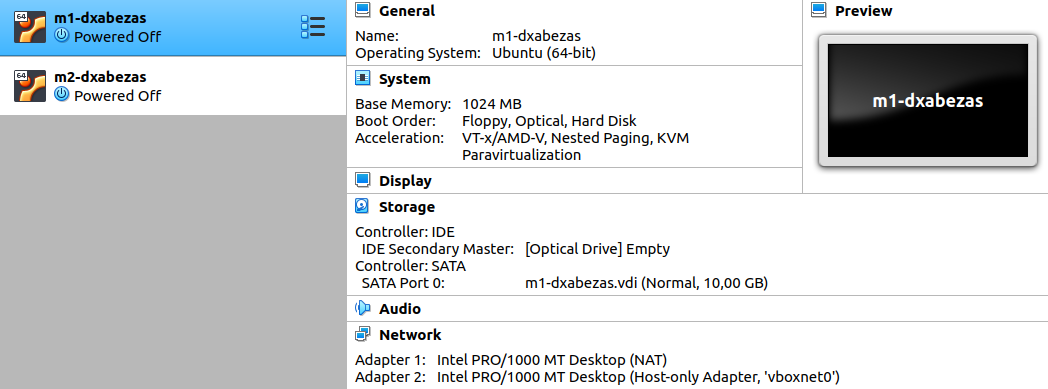
\includegraphics[width=160mm]{imgs/maquinas}
	\caption{Resumen de la configuración de la máquina M1. Observamos que tiene los dos adaptadores de red que hemos comentado.}
	\label{fig:maquinas}
\end{figure}

Seguidamente, instalamos Ubuntu Server 18.04 LTS en ambas máquinas. Podemos descargar la ISO de la página oficial. Creamos en las dos máquinas perfiles idénticos, con usuario \textbf{dxabezas} y constraseña \textbf{Swap1234}.

\begin{figure}[H]
	\centering
	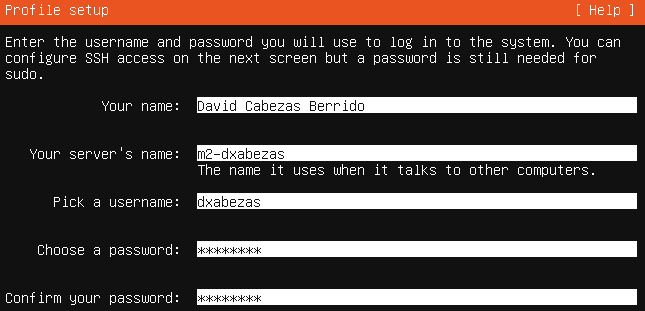
\includegraphics[width=160mm]{imgs/perfil}
	\caption{Creando el perfil en la máquina M2.}
	\label{fig:perfil}
\end{figure}

Durante la instalación escogemos siempre las opciones recomendadas, con la excepción de instalar OpenSSH.

\section{SSH}

Ya tenemos OpenSSH instalado en ambas máquinas. Si durante la instalación no lo hubiésemos marcado, tendríamos que ejecutar:

\begin{verbatim}
	sudo apt-get install openssh-client
	sudo apt-get install openssh-server
\end{verbatim}

Con \texttt{ifconfig}, podemos ver la dirección IP de cada máquina:

\begin{figure}[H]
	\centering
	\subfigure[Máquina 1.]{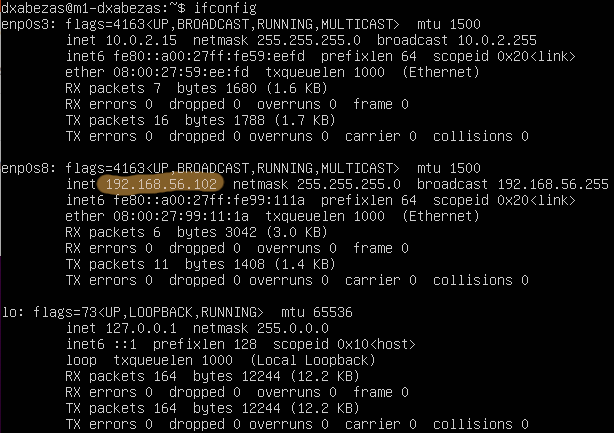
\includegraphics[width=87mm]{imgs/ifconfig1}}
	\subfigure[Máquina 2.]{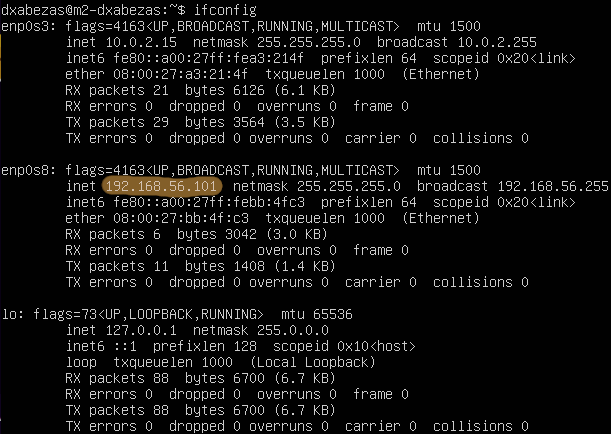
\includegraphics[width=86.5mm]{imgs/ifconfig2}}
	\caption{Direcciones IP de ambas máquinas.}
	\label{fig:ifconfig}
\end{figure}

Nos conectamos de una máquina a otra, ejecutando \texttt{ssh user@ip}.
\begin{figure}[H]
\centering
\subfigure[M1 se conecta a M2.]{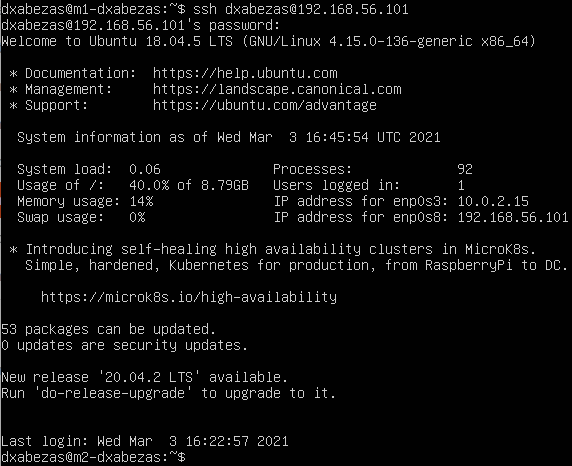
\includegraphics[width=86mm]{imgs/ssh1}}
\subfigure[M2 se conecta a M1.]{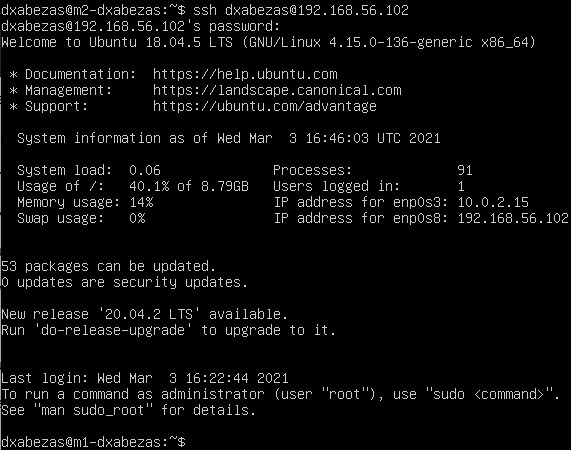
\includegraphics[width=88mm]{imgs/ssh2}}
\caption{Cada máquina se conecta a la otra por SSH con el usuario que creamos (dxabezas, Swap1234).}
\label{fig:ssh}
\end{figure}

\textbf{NOTA:} En lo que viene a continuación, la dirección IP de M1 es la que termina en 1 y la de M2 es la que termina en 2.
En la siguiente sección
explico cómo las intercambio.

Ahora vamos a configurar SSH, para ello modificamos el fichero \texttt{/etc/ssh/sshd\_config}, donde se encuentra la configuración
del servicio \texttt{ssh-server}. \texttt{/etc/ssh/ssh\_config} es para la configuración de \texttt{ssh-client}.
Por ejemplo, podemos modificar el puerto del 22 (por defecto) al 2222 con la línea \texttt{Port 2222}. Para hacer efectivos los cambios,
guardamos el archivo y reestauramos el servicio con

\begin{verbatim}
	sudo service ssh restart
\end{verbatim}

Ahora desde la otra máquina
nos conectamos, pero debemos indicar el puerto explícitamente (con la opción \texttt{-p}) al no tratarse del por defecto.

\begin{figure}[H]
	\centering
	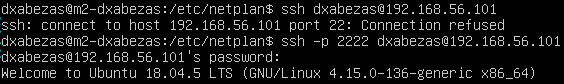
\includegraphics[width=140mm]{imgs/ssh-port}
	\caption{La máquina 2 se intenta conectar a la máquina 1. El primer intento fracasa porque intenta conectarse al puerto por defecto.}
	\label{fig:ssh-port}
\end{figure}

Una buena práctica desde el punto de vista de la seguridad es deshabilitar el root login (\texttt{PermitRootLogin no}). De esta manera,
nadie se puede conectar como root por SSH, tendrá que obtener permisos de superusuario una vez logueado en el sistema mediante sudo.

Finalmente, configuraremos el acceso sin contraseña mediante clave pública. Desde la máquina M2 generamos un par de claves con
\texttt{ssh-keygen -t rsa}, nos da la opción de poner una passphrase por si tememos que alguien pueda acceder a nuestro dispositivo.

\begin{figure}[H]
	\centering
	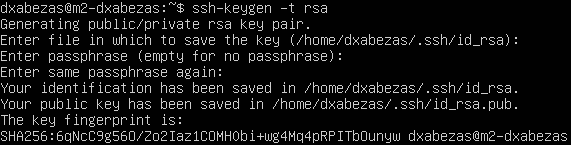
\includegraphics[width=140mm]{imgs/keygen}
	\caption{La máquina 2 genera un par de claves (pública y privada).}
	\label{fig:keygen}
\end{figure}

Ahora copiamos la clave pública en M1 ejecutando (desde M2)
\begin{verbatim}
	ssh-copy-id -p 2222 dxabezas@192.168.56.101
\end{verbatim}

nos pide la contraseña (Swap1234) y nos dice que se ha añadido 1 clave. Ahora nos podemos conectar con SSH sin poner sin que nos pida
la contraseña, nos pedirá la passphrase en caso de haber puesto una.

\section{Configuración de red}

Ya tenemos los dos adaptadores de red (NAT y Host-only) creados. Cuando instalamos el sistema se configuran por defecto,
pero podemos usar Netplan para realizar los cambios que deseemos.

Para ello, modificamos el fichero \texttt{00-installer-config.yaml} en la carpeta \texttt{/etc/netplan}, donde ya encontramos
 la configuración por defecto del adaptador NAT (interfaz \texttt{enp0s3}) y del adaptador Host-only (interfaz \texttt{enp0s8}),
 que reciben direcciones IP via DHCP. Podemos consultar las direcciones asignadas con \texttt{ifconfig} (Figura \ref{fig:ifconfig}).

\begin{Verbatim}[tabsize=4]
network:
	version: 2
	ethernets:
		enp0s3:
			dhcp4: true
		enpos08:
			dhcp4: true
\end{Verbatim}

En la Figura \ref{fig:ifconfig} también observamos que las direcciones obtenidas están ``cambiadas'', la máquina 1 recibió
 \texttt{192.168.56.102} y la máquina 2 la \texttt{192.168.56.101}. Esto se debe a que realizamos primero la instalación de la M2,
 pero ahora podemos cambiarlas manualmente para tener direcciones más intuitivas. También en la Figura \ref{fig:ifconfig} observamos
 que se utiliza la máscara de red \texttt{255.255.255.0} (24 bits a 1 y 8 bits a 0), la mantenemos añadiendo \texttt{/24} tras la dirección.
  Editamos el archivo con 
 \texttt{sudo nano 00-installer-config.yaml}. En la máquina 1 escribimos:

\begin{Verbatim}[tabsize=4]
network:
	version: 2
	ethernets:
		enp0s3:
			dhcp4: true
		enpos08:
			dhcp4: no
			addresses: [192.168.56.101/24]
\end{Verbatim}

y en la M2 cambiamos a \texttt{192.168.56.102/24}. Para aplicar los cambios ejecutamos \texttt{sudo netplan apply}, podemos comprobarlos
con ifconfig y conectarnos por ssh desde la máquina anfitriona o la otra máquina para comprobar que funciona. Si ya nos conectamos
desde la máquina anfitriona antes de este cambio, habrá que borrar la fingerprint de known hosts primero.

\begin{figure}[H]
	\centering
	\subfigure[La IP de M1 ha cambiado.]{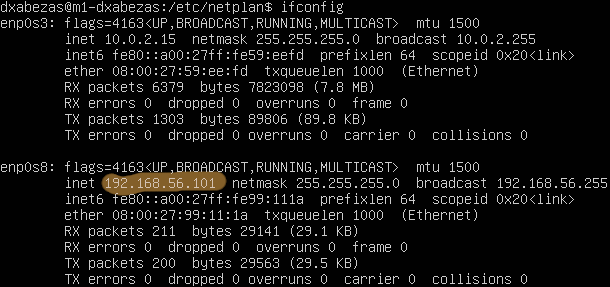
\includegraphics[width=88mm]{imgs/m1-ifconfig-static}}
	\subfigure[Nos conectamos a M1 desde el anfitrión con la nueva IP.]{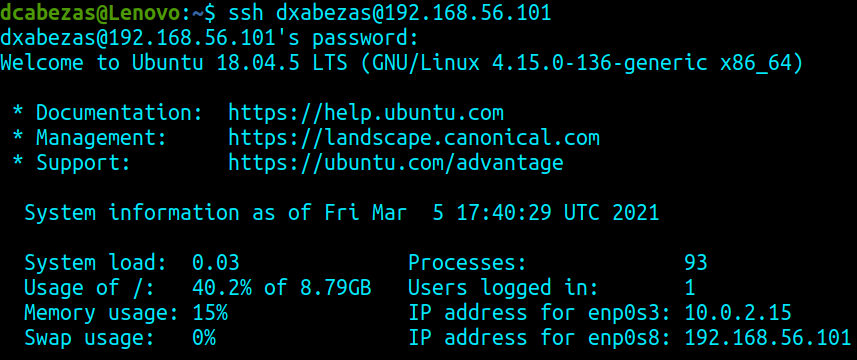
\includegraphics[width=84mm]{imgs/ssh-host}}
	\caption{Conexión por SSH desde el anfitrión a M1 con la nueva IP.}
	\label{fig:static-ip}
\end{figure}

\section{Apache2}

Puesto que no marcamos los servicios LAMP durante la instalación, debemos instalarlos manualmente. Empezamos con Apache2, en ambas máquinas ejecutamos:
\begin{verbatim}
	sudo apt install -y apache2
\end{verbatim}

Para comprobar la versión que hemos instalado usamos \texttt{apache2 -v}, y para comprobar que esté en ejecución, 
\begin{verbatim}
	sudo service apache2 status
\end{verbatim}

\begin{figure}[H]
	\centering
	\subfigure[Máquina 1.]{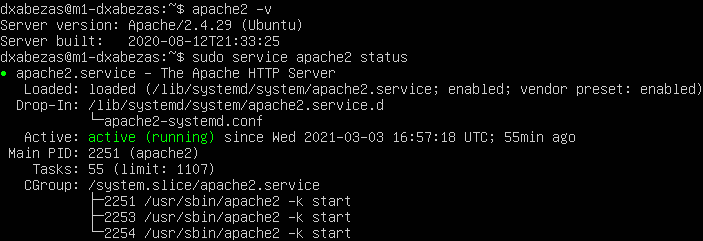
\includegraphics[width=120mm]{imgs/apache1}}
	\subfigure[Máquina 2.]{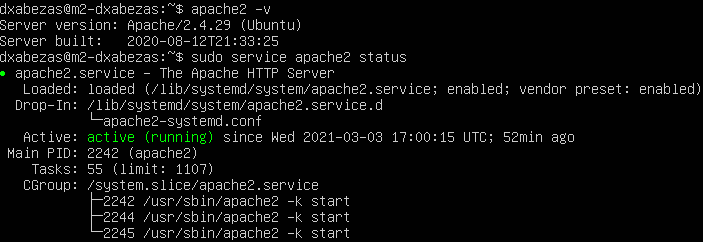
\includegraphics[width=120mm]{imgs/apache2}}
	\caption{Comprobamos la versión de Apache2 y que esté activo.}
	\label{fig:apache2}
\end{figure}



\end{document}